\subsection{Homomorphe Verschlüsselung}\label{sec:homomorphe_verschlüsselung}

Homomorphe Verschlüsselung ist eine Methodik, um Berechnung auf verschlüsselten Daten durchführen zu können. Dadurch können Daten beispielsweise in der Cloud verarbeitet werden, ohne dass es dem Anbieter des Services möglich ist, die Vertraulichkeit der Daten zu gefährden.

Ein Homomorphismus in der Algebra bezeichnet eine strukturerhaltende Abbildung einer Mengen $G$ in eine andere Menge $H$.
Dabei hat jedes Element $g \in G $ mindestens ein Bild $h \in H$ und die Relationen der Elemente $g \in G$ zueinander, finden sich auch in H wieder \cite{B-2}.

Ein typisches Beispiel ist der Homomorphismus zwischen zwei Gruppen $(G,\circ)$ und $(H,\ast)$, wobei $\circ$ und $\ast$ jeweils eine Verknüpfung innerhalb der Gruppe symbolisieren. 
Die Beziehung der beiden Gruppen wird Gruppenhomomorphismus genannt, wenn es eine Funktion $f:G\to H$ gibt, die Elemente der Gruppe $G$ auf die Gruppe $H$ abbildet und dabei für alle Elemente $g_1,g_2 \in G$ gilt \cite{P-98}:
\begin{equation*}
    f(g_1 \circ g_2) = f(g_1) \ast f(g_2)
\end{equation*}
Abbildung \ref{fig:group_homomorphismus} zeigt eine grafische Darstellung dieses Gruppenhomomorphismus.

\begin{figure}[!htb]
    \centering
    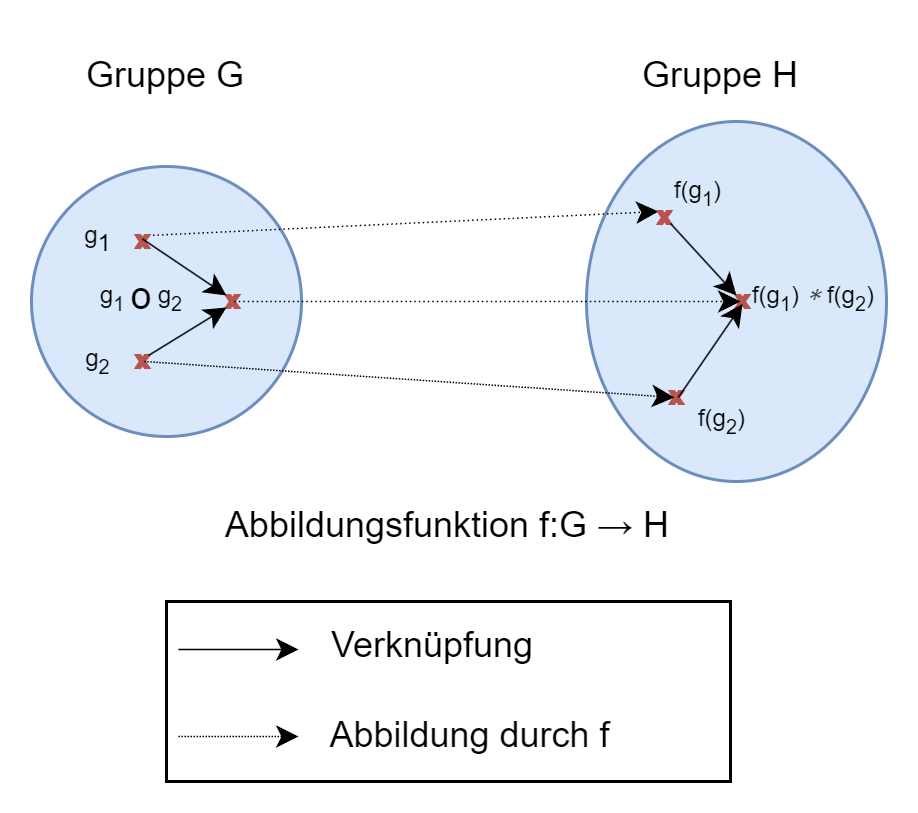
\includegraphics[width=12.5cm]{figures/group_homomophismus.png}
    \caption{Gruppenhomomorphismus nach \cite{P-98}}
    \label{fig:group_homomorphismus}
\end{figure} 

Bei der homomorphen Verschlüsselung, handelt es sich um einen Gruppenhomomorphismus zwischen der Gruppe der Klartexte $(P,\circ)$ und der Gruppe der Geheimtexte $(C,\ast)$. 
Die Abbildfunktionen sind dabei der Verschlüsselungsalgorithmus $Enc_k:P\to C$ und der Entschlüsselungsalgorithmus $Dec_k:C\to P$ mit einem Schlüssel $k \in K$ \cite{P-98}. 
Daraus lässt sich ableiten, dass folgende Bedingungen erfüllt sind:
\begin{equation*}
    Enc_k(p_1 \circ p_2) = Enc_k(p_1) \ast Enc_k(p_2) 
\end{equation*}
\begin{equation*}
Dec_k(c_1 \ast c_2) = Dec_k(c_1) \circ Dec_k(c_2)
\end{equation*}
Abbildung \ref{fig:homo_enc} zeigt, wie besagter Homomorphismus aussieht.


\begin{figure}[!htb]
    \centering
    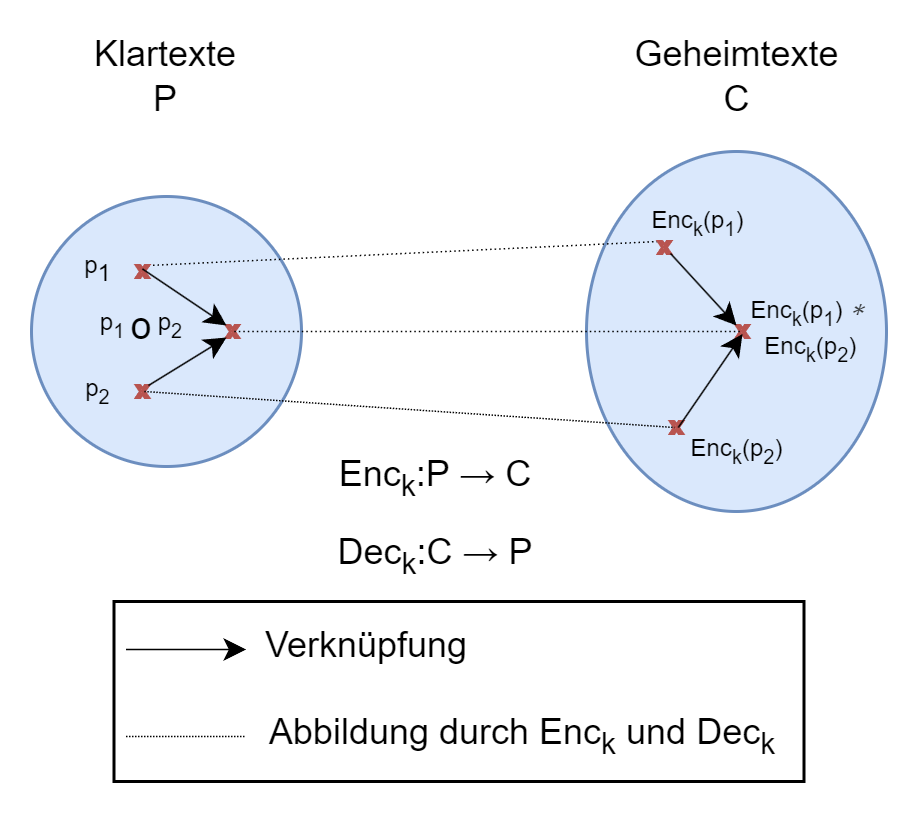
\includegraphics[width=12.5cm]{figures/homo_enc.png}
    \caption{Homomorphe Verschlüsselung}
    \label{fig:homo_enc}
\end{figure} 

Konkret bedeutet dies, dass es für eine Verknüpfung innerhalb der Gruppe der Klartexte $P$, von zwei Elemente $p_1, p_2 \in P$ auf ein drittes Element $p_3 \in P$, eine andere Verknüpfung innerhalb der Gruppe der Geheimtexte $C$ gibt, welche die gleiche Verknüpfung mit den verschlüsselten Daten berechnet. Die Verknüpfung innerhalb der Gruppe der Geheimtexte bildet also zwei Elemente $Enc(p_1), Enc(p_2) \in C$ auf ein drittes Element $Enc(p_3) \in C$ ab, welches dem verschlüsselten Wert von $p_3$ entspricht.
Ist die Verknüpfung eine Addition, so gibt es demnach die Möglichkeit, diese Addition nur mit den verschlüsselten Daten zu berechnen.

Homomorphe Verschlüsselungen lassen sich dabei in 3 Kategorien einteilen, je nachdem welche Verknüpfungen innerhalb der Gruppen möglich sind \cite{P-42}:
\begin{compactitem}
\item \textbf{Teilweise homomorphe Verschlüsselung (partially):} Entweder Multiplikation oder Addition als Verknüpfung der Klartexte möglich, jedoch nicht beides.
\item \textbf{Eingeschränkte homomorphe Verschlüsselung (somewhat oder leveled):} Sowohl Multiplikation als auch Addition möglich, jedoch beschränkt durch die Anzahl an durchführbaren Berechnungen. 
\item \textbf{Vollständige homomorphe Verschlüsselung (fully):} Multiplikation und Addition für eine unbegrenzte Anzahl an Berechnungen möglich
\end{compactitem}

Da sich die gängigsten Bestandteile eines neuronalen Netzes über Addition und Multiplikation berechnen lassen, bedeutet dies, dass das Training und auch die Inferenz eines Modells mittels homomorpher Verschlüsselung möglich ist. 

Gentry \cite{P-40} stellte 2009 das erste vollständig homomorphe Verschlüsselungssystem vor.
Dabei nutzte er eine eingeschränkt homomorphe Verschlüsselung, welche auf mathematischen Gittern basiert.
Das System war eingeschränkt homomorph, da die Verschlüsselung auf einem Rauschen basierte, welches mit jeder Operation größer wurde und letztendlich nicht mehr für eine korrekte Entschlüsselung sorgte.
Er erweiterte das System mit einer Technik namens Bootstrapping.
Dabei wird der Geheimtext ein zweites Mal verschlüsselt, sodass dieser doppelt verschlüsselt ist.
Anschließend kann mittels des verschlüsselten Schlüssels die ursprüngliche Verschlüsselung homomorph herausgerechnet werden. 
Dadurch wird das Rauschen des Verschlüsselungssystems zurückgesetzt und eine weitere Berechnung ist möglich. 
Kann das ursprünglich eingeschränkte homomorphe Verschlüsselungssystem die homomorphe Entschlüsselung und eine weitere Operation durchführen, dann kann es mittels Bootstrapping zu einem vollständig homomorphen Verschlüsselungssystem umgewandelt werden.
So nutzen beispielsweise Van Dijk \etal \cite{P-100} diesen Fakt aus, und ersetzten die auf Gittern basierte Verschlüsselung durch eine auf Ganzzahlen basierte, eingeschränkt homomorphe Verschlüsselung aus. 

Brakerski und Vaikuntanathan \cite{P-101} verbesserten die Effizienz des bereits geschilderten Ansatzes.
Sie nutzen eine eingeschränkte homomorphe Verschlüsselung auf Basis des Lernen mit Fehlern Problems (Learning with errors) zusätzlich zu einem Relinearisierungsschritt.
Dieser zusätzliche Relinearisierungsschritt reduziert die Größe des Geheimtextes, wodurch die homomorphe Entschlüsselung beim Bootstrapping vereinfacht wird.

Gentry \etal \cite{P-102} stellten eine weitere vollständig homomorphe Verschlüsselung auf Basis des Lernen mit Fehlern Problems vor.
Die darin eingesetzte, eingeschränkt homomorphe Verschlüsselung stellt den Geheimtext als eine Matrix dar.
Die Dimension der Matrix bleibt bei jeder homomorphen Operation gleich und wächst dadurch nicht.
Dies ermöglicht, den Relinearisierungsschritt zu entfernen.
Bei dem Bootstrapping bisheriger Algorithmen, musste der verschlüsselte Schlüssel oder der Public Key des Nutzers mitgeschickt werden.
Bei diesem Ansatz ist es jedoch möglich, alleine mit dem Geheimtext Operationen durchzuführen, die anschließend nur der Nutzer entschlüsseln kann.

Theoretisch wäre das Training eines neuronalen Netzes mittels vollständiger homomorpher Verschlüsselung möglich, jedoch ist es nicht praktikabel. 
Das Training besteht aus vielen Berechnungsschritten (Inferenz, Berechnen der Verlustfunktion, Gradientenberechnung, Anpassen der Gewichte), welche mit der Größe des neuronalen Netzes ansteigt.
So wird bereits bei einem neuronalen Netz mit 7 Schichten, Faltungsschichten und vollständig verbundene Schichten, die Trainingszeit auf einer gewöhnlichen CPU, von ungefähr einer Stunde auf ein ganzes Jahr erhöht \cite{P-103}.
Es ist möglich, dass weitere, verbesserte Methoden der homomorphen Verschlüsselung entdeckt werden, wodurch sich der Mehraufwand weiter reduzieren lässt und die vollständige homomorphe Verschlüsselung praktikabler wird.

Eine Alternative ist es, keine vollständige, sondern nur eine eingeschränkte homomorphe Verschlüsselung zu nutzen.
Takabi \etal \cite{P-104} zeigen, wie dies möglich ist.
Um das Problem der begrenzten Anzahl an Berechnungen von eingeschränkter homomorphen Verschlüsselung zu umgehen, wird ein zusätzlicher Schritt eingeführt. 
Wird das Rauschen der Verschlüsselung zu groß und überschreitet einen festgelegten Schwellenwert, muss der aktuelle Zustand entschlüsselt und neu verschlüsselt werden.
Hierdurch wird das Rauschen zurückgesetzt, ohne dass Bootstrapping nötig ist.
Dadurch, dass kein vollständig homomorphes Verschlüsselungssystem genutzt werden muss, können performantere, teilweise homomorphe Verschlüsselungssysteme genutzt werden.

Neben dem Training eines Modells, gibt es eine Vielzahl an Techniken, welche homomorphe Verschlüsselung nur bei der Inferenz von neuronalen Netzen nutzt. 
Diese werden in Kapitel \ref{sec:krypto_inferenz} genauer beschrieben.
Alternativ kann die homomorphe Verschlüsselung beim verteilten Lernen eingesetzt werden, was in Kapitel \ref{sec:verteiltes_lernen} beleuchtet wird. 




